\chapter{Fundamentação Teórica}

Este capítulo busca apresentar, objetivamente, as informações necessárias para a compreensão deste trabalho. Ao longo das demais seções serão abordados diversos assuntos que se relacionam com as queimadas da Amazônia e com o desafio da implementação de um modelo capaz de prever suas áreas mais suscetíveis a incêndios florestais. Para estar imerso neste conteúdo, será necessário entender a base teórica das tecnologias mais promissoras da área de aprendizado de máquina (AM), os efeitos das queimadas a longo e curto prazo e o quão importante faz-se a compreensão do ambiente para impedir ou diminuir a ocorrência destes eventos.

\section{O Bioma da Amazônia}

Os biomas, geralmente, são definidos pelas características predominantes das formações vegetais de um ambiente \cite{TIMM05}. Eles se categorizam em grandes porções geográficas que são entendidas, portanto, como grupos de organismos semelhantes que podem ser compreendidos como uma unidade, dadas as similaridades. É importante afirmar que, além desta definição, também são relevantes as formas do relevo e condições climáticas da região para conceituar um bioma.

O próprio termo ``bioma'' foi criado pelo ecólogo americano Frederic Clements (\citeyear{clements1916}), o qual foi responsável por estudar as relações existentes em comunidades vegetais e determinar que o comportamento de organismos inseridos em uma dessas comunidades busca a sua perpetuação. Este processo discorre pelo aumento das espécies e a evolução na complexidade de suas relações. O bioma é a concepção fundamental desta comunidade como uma unidade formada por partes semelhantes \cite{TIMM05}.

A compreensão da importância do bioma amazônico parte destas características. Segundo o IBGE (\citeyear{ibge04:mapabioma}), a Amazônia é o maior bioma do Brasil, ocupando um território de mais de quatro milhões de quilômetros quadrados (km²). Um terço de toda a madeira tropical do mundo está localizada na região, que abriga cerca de duas mil e quinhentas espécies de árvores e trinta mil espécies de plantas, 30\% do total existente na América do Sul.

\section{Queimadas e Incêndios Florestais}

Desde a década de 90, a região da Amazônia sofre de um  aumento em ataques e queimadas às suas áreas verdes. Segundo FEARNSIDE (\citeyear{fearnside06}), esta tendência é causada, principalmente, pelo pico de desmatamento alcançado durante a instituição do Plano Real, em 1995, e às políticas de incentivo econômico que emergiram sem uma responsabilidade ambiental adequada na mesma época. Em 2005, com a promoção da ``Operação Curupira'' atrelada às grandes taxações imbuídas às exportações internacionais, houve uma política de freio e reversão desse cenário que, contudo, não foi capaz de retrair o suficiente a média negativa dessas últimas três décadas.

As queimadas fazem parte da cultura e processo produtivo de pequenos, médios e grandes agricultores \cite{leonel00}. Trata-se de um método econômico e ágil para efetuar a limpeza de grandes pastos, remover árvores e preparar terras para o plantio. Este fenômeno se explica em seus inúmeros benefícios: as cinzas formadas no processo são ricas em nutrientes que fertilizam o solo e podem aumentar a produtividade; o fogo utilizado é capaz de estimular o crescimento de gramíneas forrageiras e matar as ervas daninhas, fatores prejudiciais para um bom cultivo \cite{sodre21}.

A maior parte dos focos de calor mapeados na Amazônia são, portanto, incidências de fogo atribuído pela ação humana. Estas práticas agropastoris que utilizam o fogo de maneira controlada são chamadas de queimadas. Por outro lado, compreende-se como incêndio florestal toda e qualquer incidência de fogo sobre uma área vegetal por meios naturais ou através da negligência dos atores humanos; denomina o processo de combustão espontânea que ocorre, em sua maioria, nos períodos de seca e estiagem de maneira abrupta e desavisada \cite{vigano17,leonel00}.

Segundo o Instituto Nacional de Pesquisas Espaciais (INPE), o Brasil registrou 131.327 queimadas florestais até o oitavo mês de 2019. Cerca de 33\% destas incidências ocorreram na Amazônia, onde foram registrados 43.573 focos. Segundo FLORENZANO (\citeyear{florenzano07}), o Brasil é o responsável por mais de trezentas mil queimadas anualmente, se contabilizados os dados desde a década de oitenta. Este trabalho que cerca o levantamento dos números das queimadas vem sendo realizado até os dias atuais em uma parceria entre o INPE e o Instituto Brasileiro do Meio Ambiente e dos Recursos Naturais Renováveis (IBAMA), por meio de um Programa de Monitoramento de Queimadas e Prevenção e Controle de Incêndios Florestais no Arco do Desflorestamento da Amazônia, também conhecido como PROARCO.

\section{Programa Queimadas}

O Programa Queimadas é um sistema de monitoramento de focos de calor em tempo real, que opera desde 1998 com imagens de satélites, dados meteorológicos e limites políticos oficiais \cite{INPE24}. Dentre as informações que podem ser extraídas estão a posição geográfica do foco, os limites territoriais que ele faz parte, a data e hora da captura, o bioma dominante, a quantidade de dias sem chuva, valor de precipitação, a potência radioativa do fogo e o risco de incêndio no momento capturado. A Figura \ref{fig:BDQueimadas} mostra todos os registros de focos de calor da America do Sul, no dia 25 de março de 2024, por volta das 12 horas no fuso horário de Brasília.

\begin{figure}[ht]
    \centering
    \includegraphics[scale=0.4]{"imagens/Programa Queimadas.png"}
    \caption{Captura de tela realizada no dia 25 de março de 2024 sobre o BDQueimadas, mostrando os focos de calor em tempo real registrados pelo satélite GOES-16 \cite{INPE24}}
    \label{fig:BDQueimadas}
\end{figure}

\section{Sensoriamento Remoto e a Tecnologia Espacial}

``Sensoriamento remoto consiste na aquisição de informação sobre um objeto sem que se entre em contato com ele'' \cite{novo10}. Segundo o autor, essa afirmação é muito ampla enquanto definição dos serviços de monitoramento remoto, dado que pode-se adquirir informação, por exemplo, de um jogo de futebol apenas ouvindo as eufóricas reações de seus espectadores. Uma concepção mais adequada seria, portanto, atribuir o sensoriamento remoto para todo tipo de processo que impõe a utilização de um dispositivo que, mediante a observação, é capaz de inferir os fenômenos que ocorrem na superfície terrestre, a partir de uma análise da interação entre as forças que o circundam (eletromagnéticos, acústicos ou potenciais) e os elementos que constituem esta superfície. O resultado imposto ao ambiente pode ser analisado com diferentes abordagens.

Exemplificando, existem sensores capazes de detectar, por exemplo, ondas sonoras: os sonares. Eles utilizam a teoria de propagação do som para determinar a localização de objetos partindo da premissa que, em meios homogêneos, o som desloca-se em velocidade constante. Portanto, é possível determinar o posicionamento de um objeto com o cálculo da diferença entre a transmissão de um pulso e sua recepção, chamada de eco.

Segundo IGOR (\citeyear{machado17:santos17}) e LIU (\citeyear{liu07}), esta metodologia encontra uma limitação dentro do escopo da tecnologia espacial. Os sensores espaciais, como satélites, restringem-se fundamentalmente às alterações que os objetos impõem ao campo eletromagnético. É apropriado dizer, portanto, que o SR\footnote[1]{Refere-se à abreviação da expressão "Sensoriamento Remoto", a qual estamos frequentemente referenciando neste capítulo.} cabe à todo processo de obtenção de informação que utiliza-se da radiação eletromagnética (REM) e de sua interação com objetos e fenômenos, uma vez que sua detecção é independente de um meio de propagação e menos propensa a ruídos.

A Figura \ref{fig:REM} acompanha a definição de Novo (\citeyear{novo01:ponzoni}), que diz que sensoriamento remoto pode ser conceituado a partir de um esquema que possui três vértices que interagem entre si a partir de uma base em comum, a REM (radiação eletromagnética).

\begin{figure}[ht]
    \centering
    \includegraphics[scale=1]{"imagens/tcc image-SR.png"}
    \caption{Representação dos pilares do Sensoriamento Remoto \cite{novo01:ponzoni}.}
    \label{fig:REM}
\end{figure}

A base de todas as técnicas utilizadas para extrair informações de objetos remotamente está representada neste esquema. A  REM está no centro por tratar do elemento de ligação entre todos os vértices. Acima, tem-se a fonte, geralmente compreendida pelo sol ou a própria terra, a depender do tipo de sensor que vai catalisar o processo de sensoriamento, sendo que toda análise realizada é constituída pela mensuração de REM. Na base inferior esquerda do triângulo está o sensor. De forma sucinta, o sensor é definido como o dispositivo utilizado para captar a REM emitida ou refletida pelo objeto alvo. Uma vez que o alvo é o outro vértice base do triângulo, da qual se pretende extrair a informação, todos se conversam a partir da radiação eletromagnética.

\subsection{Detecção de Focos de Calor}

É fundamental conceituar que os objetos presentes na superfície terrestre emitem e refletem radiação solar. A transformação dessa energia emitida em valores de temperatura é acessível utilizando modelos físicos e, assim, é possível quantificar o calor dos ambientes monitorados. O trabalho do sensoriamento remoto é identificar estes dados que, ao ultrapassar um certo limiar (definido por especialistas), passa a relacionar estas áreas como focos de calor \cite{liu07}.

Focos de calor, a princípio, não são identificados como áreas de incêndio ou queimada. Para um dado ser interpretado como tal, faz-se necessário uma série de eventos geográficos, climáticos e florestais relacionados à região, como informa o autor:

\noindent
\begin{quoting}[rightmargin=0cm,leftmargin=4cm]
\begin{singlespace}
{\footnotesize
Para que um dado foco de calor seja interpretado como um possível foco de fogo, ou ocorrência de incêndio, a informação extraída do satélite precisa ser associada a outras informações em um Sistema de Informações Geográficas (SIG). As informações relevantes a serem associadas precisam ser definidas por meteorologistas (que vão informar se uma dada região apresenta as condições de precipitação, temperatura e umidade favoráveis à ocorrência de incêndio), por Engenheiros Florestais e Biólogos (que vão informar sobre a susceptibilidade da cobertura vegetal à combustão natural ou induzida por queimadas); por Geógrafos (que vão informar sobre a distribuição de usos da terra em diferentes áreas, sobre as práticas agrícolas, culturas dominantes etc.). \cite[p. 32]{novo10}
}
\end{singlespace}
\end{quoting}

Dessa forma, é imprescindível associar não apenas os dados mais concretos e diretos, como também informações menos relevantes e obtidas através de engenharia social para tornar a base de dados mais adequada possível para a análise.

\section{Base de dados}

Uma base de dados (ou banco de dados) é uma coleção organizada de informações ou dados, geralmente armazenados eletronicamente em um sistema de computador. É ideal que estes dados sejam estruturados de forma a permitir o armazenamento, recuperação, modificação e gestão eficientes das informações.

A ideia por trás destes modelos de informação é conter uma ampla variedade de tipos de dados, incluindo textos, números, imagens, áudio, vídeos, entre outros. Esses dados podem representar informações sobre pessoas, produtos, transações, eventos, ou qualquer outra entidade do mundo real que seja relevante para a aplicação em questão.

As bases de dados podem ser organizadas de diversas maneiras, dependendo das necessidades específicas da aplicação. Os tipos mais comuns de bases de dados incluem bases relacionais, NoSQL, orientadas a objetos, distribuídas, entre outras. Cada uma delas possui suas próprias características, estruturas e modelos de armazenamento de dados. Uma estrutura extremamente eficaz para organizar os dados, utilizada principalmente para pesquisas científicas, são as chamadas estruturas de dados tabulares. Os dados tabulares são uma forma comum e eficiente de organizar informações em uma estrutura de linhas e colunas, semelhante a uma planilha.

Existem muitos motivos que justificam a utilização de dados tabulados em pesquisas. Esta forma de organização estruturada fornece um conteúdo fácil de entender, onde cada linha representa uma observação ou exemplo e cada coluna representa uma variável ou atributo. Isso auxilia a interpretação e análise dos dados. Outro fator é que estas estruturas são compatíveis com uma grande variedade de ferramentas e plataformas, o que facilita a manipulação, análise e visualização dos dados. Além disso, podem acomodar uma ampla gama de tipos de dados, incluindo números, texto, datas e categorias. Isso os torna adequados para as tarefas de análise, onde os dados tabulares podem ser facilmente compartilhados e comunicados entre diferentes partes interessadas e são visualmente claros e objetivos.

Trabalhar com dados tabulares requer habilidades em manipulação de dados, análise exploratória, entendimento conceitual dos atributos e interpretação de resultados. Ao dominar essas habilidades, é possível extrair informações valiosas e tomar decisões fundamentadas nos dados fornecidos.

\section{Técnicas de pré-processamento}

A limpeza de dados, também conhecida como pré-processamento de dados, é uma etapa fundamental em qualquer trabalho de classificação e previsão de eventos com \textit{Machine Learning} (ML). Essa etapa envolve a identificação, correção e eliminação de problemas nos dados antes de serem usados para treinar um modelo de ML. Dados sujos ou mal formatados podem prejudicar a qualidade e a precisão de um modelo. Modelos treinados com dados limpos são mais fáceis de interpretar e entender, e isso é especialmente importante em cenários onde é necessário explicar ou justificar as previsões do modelo. Por fim, outro campo altamente influenciado por dados de alta qualidade é a eficiência computacional. Em casos onde há limitação de recursos computacionais, prover dados ``limpos'' para a máquina pode reduzir radicalmente o tempo de treinamento e auxiliar na inferência do modelo.

A presença de ruído, valores ausentes, \textit{outliers} ou inconsistências nos dados pode levar a previsões imprecisas ou enviesadas, tendo um impacto direto nos resultados do modelo. Portanto, é necessário entender os principais problemas conhecidos em dados tabulares e como identificar e realizar o tratamento dos mesmos.

\subsection{Ruídos e \textit{Outliers}}

\textit{Outliers} são pontos de dados que se desviam significativamente do padrão geral de um conjunto de dados. Eles são observações que estão ``longe'' da maioria das outras observações nos dados. A presença de \textit{outliers} pode indicar uma variedade de situações, como erros de medição, flutuações naturais extremas nos dados, ou até mesmo eventos raros ou anomalias que merecem atenção especial.

Entre as principais características dos \textit{outliers} estão os valores extremos, que estão significativamente distantes dos valores típicos ou centrais do conjunto de dados. Eles podem ser muito maiores ou menores do que a maioria dos outros valores e podem distorcer os resultados estatísticos, como média e desvio padrão e, assim, influenciar negativamente a precisão e a interpretação de modelos estatísticos ou de aprendizado de máquina.

Semelhantes aos \textit{outliers}, tem-se os ruídos, que se referem a variações aleatórias ou flutuações nos dados que não estão relacionadas ao fenômeno que está sendo observado. Essas variações aleatórias podem ser introduzidas por uma variedade de razões, como erros de medição, imprecisões nos instrumentos de coleta de dados e interferência ambiental. Sendo assim, não seguem nenhum padrão discernível ou tendência. Enquanto os \textit{outliers} representam observações extremas que se desviam significativamente do padrão geral dos dados, os ruídos são variações aleatórias mais sutis que não são necessariamente extremas, mas podem contribuir para a variabilidade geral dos dados.

A identificação destes tipos de dados geralmente envolve o uso das próprias técnicas estatísticas, como a análise \textit{z-score}. Visualizações de dados, como gráficos de dispersão, histogramas e \textit{boxplots}, também podem ajudar na detecção. Contudo, é importante destacar que nem todos os dados que estão distantes ou fora do padrão consistem em \textit{outliers}. Às vezes, eles representam variações genuínas nos dados e podem conter informações valiosas para as avaliações e testes de uma máquina de aprendizado, por exemplo. Mitigar a existência desses tipos de imprecisão envolve algumas técnicas tradicionais de suavização de dados, filtragem de ruído ou até mesmo melhorias nos processos de coleta para aumentar a eficiência dos detectores e da transcrição dos dados.

\section{Imagens Digitais}

Imagens são fontes de informação visuais compostas por pixels, unidades mínimas e finitas de dados em uma grade bidimensional. Estas pequenas unidades contém valores numéricos que indicam sua cor e intensidade, sendo armazenados digitalmente. A resolução da imagem é determinada pela quantidade de pixels, que influencia na qualidade e nitidez da representação. De todas as imagens podem ser extraídas duas importantes informações: visuais e descritivas. O que ocorre é que informações descritivas remetem ao modelo matemático que define a imagem, enquanto informação visual é a representação imagética que é exibida numa tela digital \cite{scuri02}.

Ao contrário das imagens analógicas, que são registradas em meios físicos, como filmes fotográficos, as imagens digitais existem como arquivos eletrônicos. A transição para o formato digital trouxe benefícios significativos, como a facilidade de armazenamento, manipulação e compartilhamento de imagens. Além disso, as imagens digitais podem ser facilmente processadas e editadas usando \textit{software} de edição de imagem, oferecendo maior flexibilidade criativa. Outro ponto, e o mais importante para este estudo, é que as imagens digitais podem ser facilmente adequadas e utilizadas como objeto de pesquisa. O uso de imagens e fenômenos alinhados à utilização de dados precisos são poderosas ferramentas para análise e previsão de eventos, utilizando técnicas de inteligência artificial, como o aprendizado de máquinas.

\subsection{Imagens Espectrais}

O sensoriamento remoto, mais especificamente as informações oferecidas pela pesquisa advinda dos satélites que orbitam e mapeiam a superfície terrestre, é capaz de dialogar com as mais diversas áreas de análise de dados. Estes dispositivos são responsáveis pela captação em tempo real de dados descritivos e os modelos imagéticos que representam as regiões observadas, permitindo a análise e compreensão de alguns cenários ambientais \cite{fitz20}. As imagens obtidas pelos sensores espaciais possuem características que facilitam a identificação das superfícies e as situações climáticas do ambiente. São chamadas de imagens espectrais.

As imagens espectrais referem-se a representações visuais de uma cena capturada em diferentes bandas do espectro eletromagnético. Cada banda corresponde a uma faixa específica de comprimentos de onda, abrangendo desde o visível até além do infravermelho \cite{novo01:ponzoni}. Ao analisar as respostas espectrais em diferentes bandas, é possível extrair dados sobre vegetação, uso do solo, recursos naturais e mudanças ambientais. A capacidade de capturar dados em diversas partes do espectro torna as imagens espectrais ferramentas valiosas em áreas como sensoriamento remoto. A diversidade de comprimentos de onda nas imagens, incluindo o infravermelho, permite análises diferenciadas, sendo amplamente utilizadas especialmente para monitorar a vegetação. Índices de vegetação, calculados a partir das respostas espectrais, são essenciais para estudar a atividade fotossintética e a biomassa vegetal, por exemplo. A compreensão das formas de relevo, níveis de densidade florestal e atribuição de focos de calor às regiões estudadas são características valiosas que podem ser extraídas do ambientes graças a esse tipo de representação.


\section{Inteligência Artificial}

O livro \textit{Artificial Intelligence: A Modern Approach} (\citeyear{russel20}) oferece uma perspectiva abrangente sobre o surgimento e a natureza da inteligência artificial (IA). A ideia de IA surgiu no meio do século XX, concebida logo após a segunda guerra mundial, com a visão de criar sistemas capazes de realizar tarefas que, normalmente, exigiriam inteligência humana. No cerne desse conceito está a capacidade de aprender, raciocinar, perceber e interagir de maneira adaptativa com o ambiente. Atribui-se essa denominação a qualquer sistema que pode realizar a ``função ideal'' para resolver um problema, dado o que se conhece sobre um determinado processo. A busca por replicar a cognição humana e a capacidade de raciocínio lógico de maneira artificial levou a quatro categorias fundamentais na constituição de IA's, conforme delineadas no livro de Russel e Norvig \cite{russel20}.

A primeira é denominada \textit{thinking humanly}, que pode ser traduzida de forma literal para ``pensar como um humano'' e emprega a construção de sistemas que imitam os processos mentais humanos, buscando compreender e replicar a forma como os seres humanos pensam. A segunda, \textit{thinking rationally} (pensar racionalmente) centra-se na criação de agentes racionais capazes de tomar decisões lógicas e coerentes, independentemente de replicarem diretamente o pensamento humano. A terceira abordagem, \textit{acting humanly} (em português, agir como um humano) contempla a simulação de comportamentos humanos, priorizando a execução de tarefas de maneira semelhante às que são executadas por estes seres, de maneira geral, assimilando as decisões que são tomadas no mundo real e em situações específicas. Por fim, \textit{acting rationally} ou ``agir racionalmente'' é a quarta definição, que busca desenvolver agentes capazes de tomar ações que levem aos melhores resultados possíveis, alinhando-se com princípios de racionalidade e eficácia, independentemente de se assemelharem às ações humanas. Essas categorias abrangem uma diversidade de aspectos da IA, o que reflete a heterogeneidade de metas e abordagens na busca pela criação de sistemas inteligentes.

Para Pereira (\citeyear{Pereira}), à parte da categorização dos modelos de inteligência discutidos na literatura disposta acima, existem ainda três abordagens que representam diferentes perspectivas teóricas e metodológicas do enfrentamento que passamos para alcançar a inteligência artificial, são elas:
\begin{itemize}
    \item \textbf{Conexionista:} Seu princípio fundamental é a hipótese de causa-efeito, onde garante que a efetividade de um modelo capaz de precisar o funcionamento do cérebro humano será também suficiente para reproduzir a sua inteligência. A visão conexionista tende a lidar com problemas mais complexos e imprecisos, que podem ser definidos indiretamente, como o reconhecimento de padrões. Uma de suas principais contribuições para a Inteligência Artificial são as Redes Neurais (RNs).
\end{itemize}
\begin{itemize}
    \item \textbf{Simbólica:} Baseia-se na hipótese do sistema de símbolos físicos, que argumenta sobre um conjunto de estruturas simbólicas que, aliados a um conjunto de regras de manipulação para se manifestar sobre essas estruturas, seria o suficiente para criação de sistemas inteligentes. Concentra-se em problemas bem definidos, tal qual o planejamento de tarefas, e destaca-se em seu campo de contribuições o desenvolvimento dos chamados sistemas especialistas.
\end{itemize}
\begin{itemize}
    \item \textbf{Evolucionista:} Esta abordagem inspira-se na teoria evolucionista de Charles Darwin (naturalista e geólogo vivido entre os anos de 1809-1882). A hipótese que é submetida relata que sistemas inteligentes seriam modelados como uma espécie de simulação sobre a teoria de Darwin. Desenvolve a ideia da criação de uma população artificial que deve evoluir seus indivíduos aleatoriamente, de acordo com seus genes e informações base que serão utilizadas para solucionar um problema. As operações envolvidas no processo se inspiram nas interações genéticas da biologia tradicional, como recombinação e mutação, e buscam abordar uma variedade de problemas, com a premissa de que a evolução pode levar à descoberta de soluções eficazes. Os algoritmos genéticos tratam de uma área muito importante da IA.
\end{itemize}

Pereira também cita a existência de uma quarta abordagem para alcançar soluções complexas. Chamada de IA híbrida, que consiste no uso de mais de uma das abordagens acima ao mesmo tempo \cite{Pereira}.

Por muitos anos a Inteligência Artificial se viu presa em um conjunto de regras e lógica que demandavam tempo para serem codificadas e desgastava o vislumbre de uma tecnologia promissora. Se hoje pode-se presenciar a era das máquinas inteligentes, a IA deve uma grande parte desse sucesso à seu grande potencializador: o Aprendizado de Máquinas. Esta área é um subcampo da inteligência artificial que se concentra no desenvolvimento de algoritmos e técnicas que permitem aos computadores aprender a partir de dados.

A relação entre a Inteligência Artificial e seus algoritmos de aprendizagem está disposta na Figura \ref{fig:EscoposIA} \cite{goodfellow16}. O Diagrama de Venn representado nesta imagem é uma abstração de como estão dispostos os escopos de trabalho no campo da IA.

\begin{figure}[hbt]
    \centering
    \includegraphics[scale=0.5]{"imagens/Inteligência Artificial.jpg"}
    \caption{Representação dos escopos da Inteligência Artificial \cite{goodfellow16}.}
    \label{fig:EscoposIA}
\end{figure}

A camada mais externa é o conceito de inteligência artificial, que possui diversos campos de estudo e abordagens em sua busca pela simulação da inteligência humana; em seguida, o aprendizado de máquinas que nada mais é que um subconjunto da área, fundamentado em desenvolver modelos que sejam capazes de permitir que um sistema artificial aprenda padrões a partir de dados, sem programação explícita; abrangendo uma área ainda mais reduzida e específica do AM, está o aprendizado de características, que são os modelos mais recentes da área, com sistemas capazes de identificar e extrair, automaticamente, as características mais relevantes dos dados, onde se encontra última camada, chamada de Aprendizado Profundo (ou \textit{Deep Learning}). O aprendizado profundo é uma subcategoria do AM que estuda as Redes Neurais Artificiais (RNAs). Esta área de pesquisa é definida pelo uso de arquiteturas complexas de RNAs com múltiplas camadas e é, especialmente, eficaz em lidar com conjuntos de dados grandes e complexos, sendo uma das razões para sua crescente popularidade e sucesso em diversas aplicações, como tarefas de visão computacional e processamento de linguagem natural.


\subsection{Aprendizado de Máquinas}

O escopo da inteligência artificial é muito abrangente e tem crescido de maneira exponencial nas últimas décadas, multiplicando suas áreas de aplicação e as metodologias de seus modelos e sistemas. A capacidade de raciocinar é o pivô que balanceia nossas métricas enquanto seres humanos para analisar, responder e, inclusive, aprender a executar tarefas baseando-se em nossa própria experiência. Conceder esta capacidade às máquinas é um desafio recorrente de pesquisadores e estudiosos da área, que buscam simular o processamento do cérebro humano. Os eventos biológicos que ocorrem milhões de vezes em pequenos intervalos de tempo e que são o cerne do raciocínio lógico, estimam a capacidade de memória que nosso cérebro é capaz de exprimir. Nossa existência reside fundamentalmente na capacidade de resguardar experiências e ser capaz de reproduzí-las a cada novo passo para avaliar a melhor decisão, considerando possíveis erros e acertos passados \cite{cerri17}. A ideia do Aprendizado de Máquina foi assimilada desta forma. A possibilidade de criar modelos capazes de analisar suas respostas e as respostas do ambiente para cada ação e, assim, evoluir por si. Estes modelos serão extremamente úteis para realizar tarefas de classificação e agrupamento de dados utilizadas nesta pesquisa.

Os algoritmos ou sistemas que são desenvolvidos para reconhecer padrões ou realizar previsões de maneira geral, são conhecidos como modelos de aprendizado e podem ser classificados entre dois tipos, atribuídos principalmente pela forma que são arquitetados para projetar os seus resultados. Para Cerri (\citeyear{cerri17}), existe uma clara distinção entre estes processos, os quais foram conceituados na literatura como modelos descritivos e preditivos e estão delineados abaixo:

As tarefas descritivas procuram compreender e descrever padrões ou relações nos dados para fornecer \textit{insights} sobre o comportamento subjacente do sistema. Para contribuir com este contexto, faz uso de técnicas que priorizam entender a estrutura dos dados, identificar tendências ou características importantes, em vez de fazer previsões específicas. Estes modelos que não possuem dados rotulados e, portanto, não tem uma orientação bem definida de resultados são chamados de aprendizado não supervisionado.

Já os modelos preditivos visam fazer previsões ou inferências sobre resultados futuros com base em dados históricos ou entradas fornecidas. Basicamente, são algoritmos constituídos para antecipar ou estimar valores (saída), utilizando uma base de dados bem definida e processada (entrada). Dá-se o nome de Aprendizado Supervisionado aos modelos e processos que são treinados com dados rotulados, onde as entradas estão associadas a saídas conhecidas. Quanto mais alinhados estes dados estiverem, melhores deverão ser os resultados da tarefa realizada.

\subsubsection{Regressão Logística}

A regressão logística (RL) é um dos algoritmos mais utilizados na classificação de conjuntos de dados de resposta binária. A RL é definida como uma técnica de análise de dados que utiliza argumentos matemáticos na composição do relacionamento entre eventos. De modo simples e didático, pode-se dizer que um algoritmo de Regressão Logística consiste em um método estatístico que propõe uma função de relação entre pares, usada para determinar o valor dessa relação em um escopo binário: a função logística.

A função logística (ou função sigmoidal) é uma função matemática caracterizada pela sua curva em ``S'' e é utilizada dentro do espectro do aprendizado de máquinas como uma fórmula para mapear os valores de previsão em probabilidades de acontecimento, que variam de 0 (0\%) à 1 (100\%). Dessa forma, pode-se estabelecer relações entre as variáveis independentes e as classes, para classificar a probabilidade de um acontecimento. Por exemplo, dada as saídas zero (0) e um (1) - Classe 0 e Classe 1 -  na previsão de um determinado fator, se o valor da função logística para a entrada fornecida for maior que 0.5, isso representa que aquela entrada pertence à Classe 1; caso contrário, Classe 0.

A RL pode ainda ser classificada em três tipos, quanto às classes da classificação. Primeiro, a Binomial: caracteriza-se por relacionar suas variáveis de entrada a um evento binário, como zero e um, aprovado ou reprovado, entre outros; o tipo Multinomial representa os algoritmos que fazem o mapeamento de probabilidade para mais de duas variáveis dependentes sem um ordenamento entre essas variáveis, como uma classificação entre espécies de animais, por exemplo; por fim, os algoritmos ordinais, onde estão estabelecidas três ou mais variáveis dependentes que são ordenadas em sua classificação, como níveis de som - baixo, médio ou alto.

\subsubsection{ \textit{Random Forest}}

O modelo de \textit{Random Forest} (Floresta Aleatória - FA) é um algoritmo de aprendizado de máquina composto por múltiplas árvores de decisão~\cite{breiman2001random}. Portanto, a compreensão do funcionamento da Floresta Aleatória parte da compreensão dos algoritmos de árvores de decisão. O funcionamento destas árvores é baseado, como o nome sugere, na decisão de eventos. Por exemplo: um evento de ordem binária pode ou não acontecer, de acordo com algumas características do clima e do ambiente. A árvore de decisão utiliza essas características como nós e suas arestas são as decisões que são tomadas em cada instância até que se alcance os nós filhos (a decisão final - sim ou não). No escopo das FAs, as árvores de decisão são construídas de maneira aleatória, utilizando subconjuntos dos dados para mensurar partições do vetor de características, que podem ou não ser altamente relevantes para a classificação. O objetivo desse processo é introduzir uma não-linearidade nas relações para a decisão e reduzir o risco de overfitting nos modelos treinados.

\subsubsection{Support Vector Machine}

A Máquina de Vetores de Suporte (SVM) é um modelo de aprendizado de máquinas supervisionado utilizado em muitos estudos de classificação e que recorrentemente apresenta bons resultados (inserir exemplos de outros trabalhos). O SVM opera com uma função chamada de hiperplano, uma equação linear desenvolvida sob os parâmetros de entrada que tem a função de segmentar as características que se dissociam. Um hiperplano é um conceito geométrico em um espaço de dimensão N. Em um espaço bidimensional (2D), um hiperplano é uma linha reta que divide o espaço em duas regiões. Em um espaço tridimensional (3D), um hiperplano é um plano que divide o espaço em duas partes. Em geral, em um espaço N-dimensional, um hiperplano é uma superfície de dimensão N-1 que separa o espaço em duas partes. Portanto, o objetivo do algoritmo é encontrar o hiperplano ótimo que separa os pontos de dados de diferentes classificações no espaço de características. Essa função é determinada de forma a maximizar a margem entre os pontos mais próximos de diferentes classes, tornando-o eficaz para classificação.

\subsubsection{XGBoost --- Gradient Boosting otimizado}
\label{subsec:fund_xgboost}

O \emph{XGBoost} (\emph{eXtreme Gradient Boosting})~\cite{chen2016xgboost} é uma implementação otimizada do \emph{Gradient Boosting Machine}~\cite{friedman2001greedy} que se popularizou em competições de aprendizado de máquina pela sua eficiência computacional, suporte nativo a regularização \(L_1\) e \(L_2\), \emph{early stopping} e paralelização. Em essência, o algoritmo treina iterativamente novas árvores de decisão para corrigir os erros residuais das árvores anteriores, com uma função objetivo que combina perda e regularização. Cada nova árvore é construída ponderando observações que o modelo atual erra mais --- processo conhecido como \emph{boosting}. Em datasets tabulares com forte sinal não-linear, o XGBoost tipicamente supera Random Forest puro em acurácia, conforme demonstrado por Quesada-Ruiz \emph{et al.}~\cite{npjhazards2025fire} em previsão sazonal de fogo no Brasil.

\subsubsection{LightGBM --- \emph{boosting} baseado em histograma}
\label{subsec:fund_lightgbm}

O \emph{LightGBM}~\cite{ke2017lightgbm} implementa duas otimizações sobre o GBM tradicional: \emph{(i)} \emph{histogram-based learning}, em que valores contínuos são pré-discretizados em \emph{bins}, reduzindo significativamente o custo de busca por divisões (\emph{splits}) ótimas; \emph{(ii)} \emph{leaf-wise tree growth} (em oposição ao \emph{level-wise} tradicional), em que cada iteração expande o nó folha que mais reduz a perda, gerando árvores mais profundas e específicas. O resultado prático é treinamento entre cinco e dez vezes mais rápido que o XGBoost em \emph{datasets} grandes, com acurácia equivalente ou superior. A contrapartida é o maior risco de \emph{overfitting} em \emph{datasets} pequenos, mitigado pelo controle dos parâmetros \texttt{min\_child\_samples} e \texttt{num\_leaves}.

\subsubsection{CatBoost --- \emph{boosting} nativo para \emph{features} categóricas}
\label{subsec:fund_catboost}

O \emph{CatBoost}~\cite{prokhorenkova2018catboost} endereça uma limitação dos GBMs anteriores: a necessidade de pré-codificação das \emph{features} categóricas via \emph{one-hot encoding} ou similar, que infla a dimensionalidade e gera viés de \emph{target leakage} quando o \emph{encoding} usa estatísticas do alvo. O CatBoost incorpora codificação categórica baseada em \emph{ordered target statistics}, que evita esse vazamento. Também oferece \texttt{auto\_class\_weights='Balanced'} de forma nativa para \emph{datasets} desbalanceados, o que o torna conveniente como \emph{base learner} em \emph{pipelines} de risco de fogo.

\subsubsection{\emph{Ensembles} --- \emph{Voting} e \emph{Stacking}}
\label{subsec:fund_ensembles}

O conceito de combinar múltiplos modelos em um \emph{ensemble} foi formalizado por Wolpert~\cite{wolpert1992stacked} sob o nome \emph{Stacked Generalization}. A ideia central é que diferentes algoritmos exploram diferentes regiões do espaço de hipóteses; combinar suas saídas reduz a variância e o viés do classificador final. Duas estratégias são adotadas no presente trabalho:

\begin{itemize}
  \item \textbf{\emph{Voting Soft}}: cada modelo base produz probabilidades para cada classe; a predição final é a classe com a maior probabilidade média entre os modelos. Funciona melhor que \emph{hard voting} (média de classes preditas) porque preserva a incerteza dos modelos individuais.
  \item \textbf{\emph{Stacking}}: as probabilidades dos modelos base servem como \emph{features} para um \emph{meta-classificador} que aprende a melhor combinação. Diferente do \emph{Voting}, o \emph{Stacking} pode aprender que certos modelos são mais confiáveis para certas classes. O meta-classificador costuma ser um modelo mais simples (Regressão Logística) para evitar \emph{overfitting}, mas modelos mais expressivos como \emph{Gradient Boosting}~\cite{friedman2001greedy} podem ser usados quando há volume suficiente de dados --- escolha adotada neste trabalho com ganho de 1~pp em acurácia (Capítulo~\ref{cap:resultados}).
\end{itemize}

\subsection{Reconhecimento de Padrões}

``Reconhecimento de padrões é a transformação da informação do nível subsimbólico (sinais) para o nível simbólico (o do conhecimento)'' \cite[p.15]{Babini07}. Para Babini, os modelos de classificação de modo geral executam um processo composto por alguns passos sequênciais para atingir seus objetivos, denominado reconhecimento de padrões. Os algoritmos devem partir de um extrator de características, onde obtém informações genéricas sobre os dados de entrada para definir os rótulos das saídas; o que se sucede é o seletor de características, para o qual é atribuída a tarefa de extraír novas características dos dados, desta vez com o objetivo discriminar estes dados para o próximo passo; por fim, o classificador, a última etapa de reconhecimento de padrões, que utiliza um algoritmo de aprendizado de  características e os dados discriminados atribuir para as classes.

As Redes Neurais Artificiais (RNAs) representam um subconjunto do aprendizado de máquinas que está intrinsicamente ligado aos algoritmos de aprendizado profundo. Magro (\citeyear{Magro21}) atribui que, resumidamente, as Redes Neurais Artificiais foram desenvolvidas para simular as Redes Neurais Biológicas quanto às relações entre neurônios - que foram reproduzidos computacionalmente como nós - e os processos de sinapse, para a comunicação e transmissão de sinais entre os mesmos. Assim como funciona o nosso cérebro, é centrado na ideia de aprendizado através de treinamento, sendo capaz de responder a estímulos incitados durante o mesmo. Na literatura, RNAs são utilizadas para muitos processos, inclusive, o reconhecimento de padrões.

``A transmissão do sinal de um neurônio a outro no cérebro é um processo químico complexo, no qual substâncias específicas são liberadas pelo neurônio transmissor. O efeito é um aumento ou uma queda no potencial elétrico no corpo da célula receptora. Se este potencial alcançar o limite de ativação da célula, um pulso ou uma ação de potência e duração fixa é enviado para outros neurônios'' \cite{Barioni17}. Na definição biológica, o neurônio passa a estar ativado. O processo artificial acontece de forma análoga, os neurônios atuam como unidades de processamento (nós) e estão distribuidos em camadas interconectadas. Apenas as camadas consecutivas possuem conexão direta, para as quais são atribuídos pesos, distinguindo-se como camada de entrada (nós iniciais), camada intermediária ou oculta (nós intermediários, que podem conter uma ou mais camadas) e camada de saída, que discriminam os nós de saída.

Para cada conexão entre neurônios é associada a um peso. A entrada é multiplicada pelo peso associado a cada conexão, e esses valores ponderados são somados. Esse resultado é então submetido a uma função de ativação, que determina se o neurônio deve ser ativado ou não. O processo é repetido através das camadas da rede até que a saída desejada seja alcançada. A função de ativação é crucial para introduzir não-linearidades na rede, permitindo que ela aprenda padrões complexos e relações não lineares nos dados.

\subsection{Aprendizado de Características e Profundo}

O conhecimento formal é mais complexo para os seres humanos do que para as máquinas \cite{goodfellow16}. A compreensão que o cérebro desempenha intuitivamente, como reconhecer um rosto em uma imagem ou falas em um áudio, tem sido o maior desafio da inteligência artificial desde a introdução desta tecnologia. É indubitável que estas questões não possuem um tratamento formal, uma vez que trata do subjetivo e, portanto, torna-se um desafio ainda maior ensinar, matematicamente ou através de regras, um computador a desenvolver esta capacidade.

Quando o Deep Blue, sistema de xadrez computacional desenvolvido por uma equipe de pesquisadores da IBM, obteve êxito na sua perfomance contra o atual campeão mundial Garry Kasparov, em 1997, acreditava-se que a máquina brevemente substituiria o homem em muitas das nossas funções \cite{deepblue02}. Algo que passou desapercebido nesta equação foi a necessidade de conhecer o mundo e não apenas uma série de lógicas lineares que geram um resultado. O escopo de aprendizado ainda era muito limitado.

Por ironia do destino, como citado anteriormente, as tarefas formais que estão entre os maiores desafios para os seres humanos acabam por ser as mais fáceis para um computador. Há muitos anos as máquinas apresentam a capacidade de superar até mesmo o melhor jogador de xadrez do mundo, mas apenas há pouco tempo tem sido capazes de se aproximar dos desempenhos de um humano médio na fala ou reconhecimento de objetos. Estas dificuldades culminaram na introdução de mecanismos capazes de extrair padrões de dados e aprender com eles. Os algoritmos que sucederam o surgimento do aprendizado de máquina, como naive bayes e regressão logística, são artefatos muito interessantes mas que dependem fortemente de uma representação de dados consistente.

Estes métodos atuam de modo geral ``projetando o conjunto certo de características a serem extraídas para essa tarefa e, em seguida, fornecendo essas características a um algoritmo de aprendizado de máquina simples'' \cite[p.3]{goodfellow16}.: a representação de imagens. De modo simples e objetivo, até então os dados de entrada eram a base para um objetivo - por exemplo: identifique que isto é um incêndio, sabendo que um incêndio tem estas características. A nova abordagem sugeriu a seguinte ideia: aprenda os traços que configuram um incêndio a partir das características que você conseguir identificar nas imagens de entrada e, com isso, melhore sua habilidade na identificação de incêndios. Dessa forma, a máquina passou a obter cada vez mais responsabilidade e o programador, menos. Contudo, representação de imagens não satisfaz todos os problemas para os quais é submetida. Por vezes, é quase tão difícil obter uma representação fiel quanto resolver o próprio problema. A resposta desenvolvida na literatura para superar estes problemas sustenta-se na hierarquia de conceitos, base para o que chamamos de Aprendizado Profundo.

Como descreve Goodfellow (\citeyear{goodfellow16}), a prescindibilidade de expressar formalmente o conhecimento é essencial para aprimorar uma inteligência artificial. Quanto mais a operação humana desconecta-se do processo, significa que nos aproximamos mais da obtenção de êxito na criação de agentes verdadeiramente inteligentes, uma vez que sua evolução deve culminar na total independência da ação humana. Conceitualmente, o aprendizado profundo fundamenta-se da ideia de que a máquina seja capaz de aprender conceitos complexos interconectando ideias mais simples, construindo conceitos uns sobre os outros, de onde vem o nome deste tipo de aprendizado. Barioni (\citeyear{Barioni17}) descreve o aprendizado profundo como:

\noindent
\begin{quoting}[rightmargin=0cm,leftmargin=4cm]
\begin{singlespace}
{\footnotesize
Aprendizagem profunda é o termo usado para denotar o problema de treinar redes neurais artificiais que realizam o aprendizado de características de forma hierárquica, de tal forma que características nos níveis mais altos da hierarquia sejam formadas pela combinação de características de mais baixo nível [3, 4, 5, 6, 7, 8]. Muitos problemas práticos têm sido resolvidos por redes neurais compostas de uma única camada intermediária [9].De fato, o Teorema da Aproximação Universal [10] garante que redes neurais com uma única camada oculta são aproximadores universais, i.e., são estruturas capazes de aproximar qualquer função contínua, contanto que se possa definir a quantidade suficiente de neurônios nessa única camada intermediária. \cite[p. 58]{Barioni17}
}
\end{singlespace}
\end{quoting}

\section{Otimização de hiperparâmetros com Optuna}
\label{sec:fund_optuna}

Modelos de aprendizado de máquina possuem hiperparâmetros --- escolhas estruturais que não são aprendidas dos dados (por exemplo \texttt{n\_estimators}, \texttt{max\_depth}, \texttt{learning\_rate}). A escolha manual desses valores (``ajuste por intuição'') é subótima; a \textbf{otimização bayesiana} explora o espaço de hiperparâmetros de forma sistemática.

O \emph{Optuna}~\cite{akiba2019optuna} implementa \emph{TPE} (\emph{Tree-structured Parzen Estimator}), um algoritmo de otimização bayesiana que modela \(P(\text{hiperparâmetros} \mid \text{resultado bom})\) e \(P(\text{hiperparâmetros} \mid \text{resultado ruim})\) separadamente, sugerindo o próximo conjunto de hiperparâmetros que maximiza a razão entre essas duas distribuições. Neste trabalho, o Optuna foi aplicado em quatro modelos (RF, LR, XGBoost, LightGBM), cada um com 15 \emph{trials} e validação cruzada estratificada em três \emph{folds}, otimizando \(\text{F}_1\)-macro. Os ganhos foram substanciais: XGBoost \(+8,4\,\text{pp}\) em \(\text{F}_1\)-macro CV; LightGBM \(+5,5\,\text{pp}\); RF \(+4,5\,\text{pp}\).

\section{Interpretabilidade de modelos}
\label{sec:fund_interpretabilidade}

Modelos de \emph{ensemble} e \emph{boosting} funcionam como \emph{black boxes}: alta acurácia, baixa transparência. Para uso em decisões de gestão ambiental --- objetivo deste TCC --- é fundamental que o sistema \textbf{explique por que} classificou um ponto como de risco ``Muito Alto''. Duas técnicas modernas são adotadas neste trabalho:

\paragraph{SHAP (\emph{SHapley Additive exPlanations})~\cite{lundberg2017unified}.} Baseado em teoria dos jogos cooperativos (valores de Shapley), atribui a cada \emph{feature} uma contribuição numérica para a predição individual, de modo que a soma das contribuições reconstitui a probabilidade predita. Para modelos baseados em árvores, há uma implementação exata em tempo polinomial denominada \emph{TreeExplainer}~\cite{lundberg2020local}. O cálculo de SHAP por classe permite identificar quais \emph{features} dirigem cada uma das 3 classes de risco separadamente.

\paragraph{\emph{Permutation Importance}~\cite{breiman2001random,fisher2019all}.} Formaliza a importância de uma \emph{feature} como a degradação esperada da métrica de avaliação (\(\text{F}_1\)-macro, \(\text{F}_1\) por classe) quando os valores da \emph{feature} são permutados aleatoriamente, mantendo a distribuição marginal. É \emph{model-agnostic} (funciona com qualquer modelo) e não enviesada para \emph{features} de alta cardinalidade~\cite{strobl2007bias} --- propriedade relevante quando há OHE de variáveis como \texttt{Municipio} (542 categorias) ou \texttt{Estado} (9 categorias) pós-OHE. A análise complementar via importância \emph{condicional}~\cite{hooker2021unrestricted} é apontada como trabalho futuro no Capítulo~\ref{cap:conclusao}, dada a multicolinearidade nas \emph{features} de janela móvel.

Molnar~\cite{molnar2022interpretable} oferece tratamento aprofundado de ambas as técnicas, incluindo limitações práticas (e.g.\ \textsection~8.5 sobre multicolinearidade na \emph{Permutation Importance}) que pautaram as decisões do Capítulo~\ref{cap:resultados}.

\section{Tratamento de desbalanceamento de classes}
\label{sec:fund_desbalanceamento}

Em \emph{datasets} reais, classes raras são tipicamente minoritárias, e modelos treinados sem mitigação tendem a privilegiar as classes majoritárias~\cite{he2009learning}. Três estratégias foram avaliadas neste trabalho:

\begin{enumerate}
  \item \texttt{class\_weight='balanced'}: cada classe contribui para a função de perda com peso inversamente proporcional à sua frequência. Não cria amostras sintéticas; apenas re-pondera. É a estratégia adotada nos modelos finais \texttt{random\_forest\_balanced} e \texttt{logistic\_regression\_balanced}.

  \item \textbf{SMOTE} (\emph{Synthetic Minority Over-sampling Technique})~\cite{chawla2002smote}: gera amostras sintéticas da classe minoritária interpolando vizinhos. Aumenta o suporte de classes raras, mas pode criar exemplos não-realistas em \emph{datasets} com forte estrutura espacial-temporal. Foi implementada com a biblioteca \emph{imbalanced-learn}~\cite{lemaitre2017imbalanced} na variante \texttt{random\_forest\_smote}.

  \item \textbf{\emph{Threshold tuning} multi-classe}: em vez de aplicar \texttt{argmax} sobre as probabilidades calibradas, ajustam-se limiares \(\bigl(\text{thr}_{\text{Mod}}, \text{thr}_{\text{MuitoAlto}}\bigr)\) que privilegiam a revocação da classe minoritária, maximizando \(\text{F}_1\) na classe \emph{Moderado} sem custo de \(\text{F}_1\)-macro global.
\end{enumerate}

\section{Calibração de probabilidades}
\label{sec:fund_calibracao}

A predição padrão dos modelos retorna escores não-calibrados --- em particular, Random Forest e GBMs tendem a produzir probabilidades subestimadas próximas a 0 e superestimadas próximas a 1. Para que a saída do modelo seja interpretável como ``\(P(\text{classe} \mid \text{features}) = 0{,}73\)'', é necessário aplicar uma transformação de calibração após o treinamento.

Duas técnicas clássicas existem: a calibração de Platt~\cite{platt1999probabilistic}, que ajusta uma sigmoide entre os escores brutos e a probabilidade empírica; e a calibração isotônica~\cite{zadrozny2002transforming}, que ajusta uma função monotônica não-paramétrica sem assumir forma sigmoidal. A última é a adotada neste trabalho via \texttt{CalibratedClassifierCV} do \emph{scikit-learn}~\cite{pedregosa2011scikit}, com validação cruzada em 3 \emph{folds} para evitar \emph{overfitting} da calibração.

\section{Índices físico-climáticos de fogo}
\label{sec:fund_indices_fogo}

A literatura de risco de incêndio acumulou, desde os anos 1960, um conjunto de índices físicos para quantificar \textbf{déficit hídrico}, \textbf{estresse atmosférico} e \textbf{aridez}. Quatro deles são adotados neste trabalho como \emph{proxies} à variável \texttt{Umidade} (cuja integração via NASA POWER é cara em tempo):

\begin{description}
  \item[KBDI (\emph{Keetch-Byram Drought Index})~\cite{keetch1968drought}.] Integral acumulada de déficit de evapotranspiração; alta em períodos secos prolongados e baixa após chuvas. Identificado por Vasconcelos \emph{et al.}~\cite{forests2024cerradoamazon} como o melhor preditor de fogo em Canaã dos Carajás, no Pará, e portanto altamente relevante para o presente estudo.

  \item[SPI (\emph{Standardized Precipitation Index})~\cite{mckee1993spi}.] Padroniza a precipitação acumulada em janelas (1, 3, 6, 12 meses) sobre a climatologia local. \(\text{SPI} < -1\) indica seca; \(\text{SPI} > +1\) indica regime chuvoso. Quesada-Ruiz \emph{et al.}~\cite{npjhazards2025fire} demonstraram que o SPI observado prevê anomalia de área queimada com até um mês de antecedência em \(\approx 68\%\) das áreas queimáveis brasileiras.

  \item[VPD \emph{proxy} (\emph{Vapor Pressure Deficit})~\cite{seager2015climatology}.] Mede a capacidade absoluta da atmosfera de extrair água da superfície. Seager \emph{et al.} demonstram que o VPD é superior à umidade relativa isolada como métrica de risco de fogo.

  \item[Aridez de De Martonne~\cite{demartonne1926aridity}.] Índice clássico \(P / (T + 10)\) baseado em precipitação anual e temperatura média; permite estratificação regional do risco em escala anual.
\end{description}

\section{Validação temporal de modelos}
\label{sec:fund_validacao_temporal}

Em \emph{datasets} com componente temporal, a divisão clássica \texttt{train\_test\_split(stratify=y)} mistura observações de todos os anos entre treino e teste. Quando o \emph{pipeline} computa \emph{features} de janela móvel (por exemplo \texttt{Precipitacao\_ma90}, \texttt{SPI\_3m}, \texttt{Incendios\_Ultimos\_180\_Dias}) sobre o \emph{conjunto inteiro antes do} \emph{split}, há risco de \textbf{vazamento temporal}: linhas de teste podem ter recebido contribuição estatística de linhas próximas no espaço-tempo que estão no treino. Esse efeito \textbf{superestima} a capacidade preditiva real do modelo em um cenário causal estrito~\cite{bergmeir2012cv}.

A solução é o procedimento \emph{rolling-origin} por ano: para cada ano \(Y\) entre os três últimos com massa suficiente, treina-se em observações com \(\text{Ano} < Y\) e testa-se em observações com \(\text{Ano} = Y\). Simula o uso real: ``treine com tudo até hoje, prediga o ano seguinte''. Aplicada ao modelo final neste trabalho, revela uma queda de \SI{14,49}{pp} em acurácia e \SI{32,35}{pp} em \(\text{F}_1\)-Moderado (Capítulo~\ref{cap:resultados}) --- valores que são reportados explicitamente para balizar a interpretação das métricas do \emph{split} aleatório.

\subsection{Métricas de Avaliação}

Uma das decisões mais importantes e essenciais para realizar previsões consistentes é definir a metodologia adotada para avaliar os resultados apresentados pela máquina. Não existe uma regra linear para definir as métricas de avaliação de um modelo proposto. As funções e abordagens que podem ser utilizadas dependem essencialmente do próprio modelo de aprendizado, bem como do tipo do problema definido e dos dados de entrada da máquina.

Quando um modelo de classificação faz previsões sobre um conjunto de dados, ele atribui uma classe a cada exemplo de dados com base em suas características. Essas classes atribuídas pelo modelo são as "classes preditas". Para avaliar a precisão do modelo, precisamos comparar suas previsões com a verdadeira classe de cada exemplo de dados. Essas são as "classes verdadeiras" ou "rótulos verdadeiros" de cada exemplo, que são conhecidos antes de realizar as previsões do modelo. Existem diferentes formas de fazer essa aproximação, mas todas compartilham um objetivo em comum: medir quão distante o modelo está da classificação perfeita.

A matriz de confusão é uma ferramenta essencial para avaliar o desempenho de um modelo de classificação. Consiste em uma tabela que mostra a frequência com que as previsões do modelo são corretas ou incorretas em relação às classes reais dos dados. A matriz de confusão é especialmente útil quando se trata de problemas de classificação com mais de duas classes. A figura 4 apresenta a representação visual desta matriz, sendo uma tabela onde as classes reais estão dispostas nas suas linhas e as classes previstas pelo modelo são representadas nas colunas. A matriz é dividida em quatro células: Verdadeiros Positivos (TP), Falsos Positivos (FP), Verdadeiros Negativos (TN) e Falsos Negativos (FN).

\begin{figure}[ht]
    \centering
    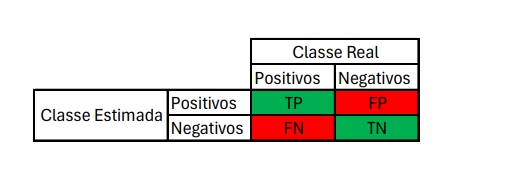
\includegraphics{imagens/TCC-MC.png}
    \caption{Representação gráfica de uma matriz de confusão}
\end{figure}

Contudo, precisamos entender os conceitos atribuídos à cada uma dessas definições. Verdadeiros positivos são as ocorrências em que o modelo previu corretamente a classe positiva. Em outras palavras, são instâncias que realmente pertencem à classe positiva e o modelo as classificou corretamente como positivas. Falsos positivos são atribuídos aos casos em que o modelo previu incorretamente a classe positiva. Ou seja, são instâncias que na verdade pertencem à classe negativa, mas o modelo as classificou erroneamente como positivas. Os verdadeiros negativos introduzem ocorrências em que o modelo previu corretamente a classe negativa. São instâncias que realmente pertencem à classe negativa e o modelo as classificou corretamente como negativas. Por fim, falsos negativos remetem aos casos em que o modelo previu incorretamente a classe negativa. Ou seja, são instâncias que na verdade pertencem à classe positiva, mas o modelo as classificou erroneamente como negativas.

Estas frequências são fundamentais para entender o funcionamento do modelo. A partir da matriz de confusão, é possível calcular calcular métricas de desempenho como precisão, recall, F1-score e taxa de erro, utilizando a proporção destas ocorrências. A interpretação da matriz ajuda a entender os pontos fortes e fracos do modelo e pode orientar ajustes para melhorar sua performance.

\subsubsection{Precisão}

A métrica de precisão (ou acurácia) é uma medida que avalia a proporção de instâncias classificadas corretamente como positivas em relação ao total de instâncias classificadas como positivas, tanto corretamente quanto incorretamente. Matematicamente, a precisão é calculada pela fórmula:

\[
    Precisao = \frac{TP}{TP+FP}
\]

Essencialmente, a precisão indica a habilidade do modelo em classificar corretamente as instâncias positivas e é uma das métricas importantes para avaliar o desempenho de modelos de classificação. Neste cálculo, é considerada a proporção de exemplos corretamente classificados para uma determinada classe em relação ao total de exemplos dessa mesma classe. Em outras palavras, a métrica de precisão é constituida pela fração de previsões corretas em relação ao total de previsões feitas para uma classe específica.


\subsubsection{recall}

O recall, também conhecido como sensibilidade ou taxa de verdadeiros positivos, é outra das métricas mais utilizadas para avaliar o desempenho de modelos de classificação. Ele mede a proporção de exemplos positivos corretamente identificados pelo modelo em relação ao total de exemplos que realmente pertencem à classe positiva. É descrito pela relação:

\[
    Recall = \frac{TP}{TP+FN}
\]

Em outras palavras, o recall indica a capacidade do modelo em identificar corretamente todos os exemplos da classe positiva. Ele é especialmente importante em situações onde a identificação correta dos exemplos positivos é crucial, como em problemas de detecção de doenças, segurança e detecção de fraudes.

\subsubsection{F1-score}

Tanto a precisão quanto o recall têm como objetivo avaliar a capacidade de um modelo de classificação em identificar corretamente os exemplos positivos de uma classe. No entanto, a diferença fundamental entre essas duas métricas está na ênfase que cada uma dá a diferentes aspectos da classificação.

A precisão se concentra na proporção de exemplos classificados como positivos pelo modelo que são realmente positivos. Em outras palavras, a precisão mede a precisão das previsões positivas do modelo, ou seja, quantas das previsões positivas foram realmente corretas. Ela responde à pergunta: "De todos os exemplos classificados como positivos pelo modelo, quantos foram classificados corretamente como positivos?".

Por outro lado, o recall se concentra na proporção de exemplos positivos que foram corretamente identificados pelo modelo em relação ao total de exemplos positivos na base de dados. Em outras palavras, o recall mede a sensibilidade do modelo em detectar exemplos positivos, ou seja, quantos dos exemplos positivos reais o modelo conseguiu identificar corretamente. Ele responde à pergunta: "De todos os exemplos que realmente pertencem a uma determinada classe positiva, quantos o modelo conseguiu identificar?".

O F1-score é uma métrica que combina ambos em um único número, fornecendo uma medida geral do desempenho de um modelo de classificação. Ele é especialmente útil quando temos um desequilíbrio entre as classes do conjunto de dados.

O F1-score é calculado como a média harmônica da precisão e do recall e é definido pela seguinte fórmula:

\[
    F1 = 2*\frac{Precisao * Recall}{Precisao+Recall}
\]

Essencialmente, o F1-score fornece uma maneira de equilibrar a precisão e o recall, pois dá mais peso às classes que têm menor representação no conjunto de dados. Isso é importante porque, em conjuntos de dados desbalanceados, a precisão pode ser alta simplesmente devido à alta proporção de exemplos negativos, enquanto o recall pode ser baixo devido à baixa taxa de detecção dos exemplos positivos.

Um F1-score alto indica um equilíbrio entre precisão e recall, enquanto um F1-score baixo indica que o modelo está tendendo para um dos dois extremos.

\chapter{METODOLOGIA}
\label{cap:metodologia}

